
\section{Introduction}
\subsection{What's Software Engineering?}
Software Engineering is a branch in the field of Computer Science that revolves around designing, testing, coding, and  maintaining high-quality software 
while being able to understand the needs of the client.

\subsection{What's the Difference Between a Programmer and a Software Engineer?}
People often confuse a programmer with a software engineer. While it is true that both write code for software, a software engineer is a step ahead 
of the programmer. Not only does the engineer program, but they also possess non-technical skills that allow them to understand and guide the client 
according to their needs, create the architecture of the software, and apply various techniques and methodologies for well-structured software. 
In other words, a programmer $\subset$ software engineer.\\
\begin{center}
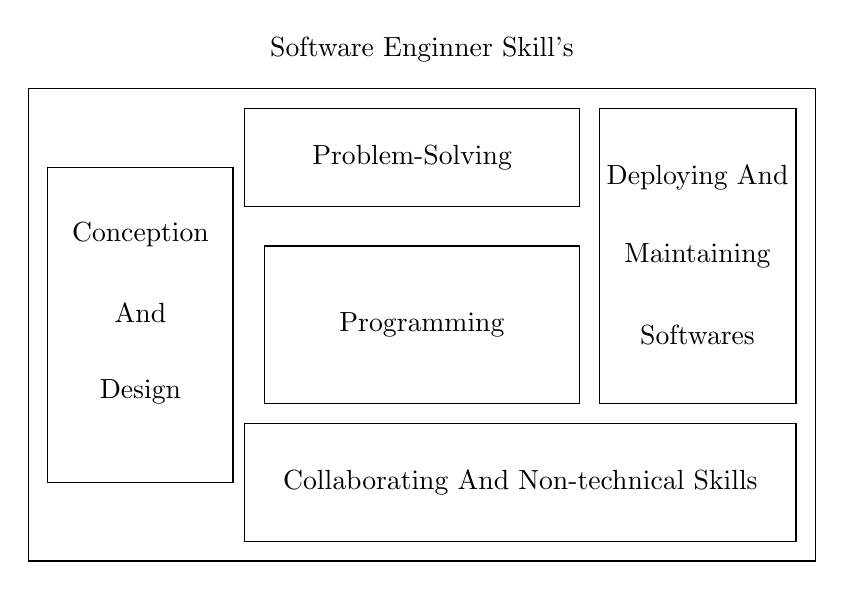
\begin{tikzpicture}
\draw (0,0) rectangle (10,6);
\node [anchor = center] at (5,6.5) {Software Enginner Skill's};

\draw (0.25,1)rectangle (2.60,5);
\node at (1.425,4.15) {Conception};
\node at (1.425,3.15) {And};
\node at (1.425,2.15) {Design};

\draw (3,2) rectangle (7,4);
\node [anchor = center] at (5,3) {Programming};

\draw (2.75,4.5) rectangle (7,5.75);
\node at (4.875,5.125) {Problem-Solving};

\draw (2.75,0.25) rectangle (9.75,1.75);
\node [anchor = center] at (6.25,1) {Collaborating And Non-technical Skills};

\draw (7.25,2) rectangle (9.75,5.75);
\node at (8.5,4.875) {Deploying And};
\node at (8.5,3.875) {Maintaining};
\node at (8.5,2.875) {Softwares};

\end{tikzpicture}
\end{center}














